\chapter{Desarrollo}

\section{Primera Iteración}

\subsection{Extracción de Texto de los Documentos del Marco Normativo}

Como se mencionó en la sección \ref{subsec:marco-normativo-ipn}, el IPN ofrece accesibilidad al conjunto de documentos que conforman el marco normativo. Existe un problema en utilizar estos documentos como fuente de información para el sistema propuesto en este trabajo terminal: \textbf{la divulgación de estos documentos se hacen en formato PDF}. Los formatos PDF agregan un formato de organización gráfica iy visual, pero no son óptimos para procesos de extracción.


\begin{figure}[ht]
    \centering
    \fbox{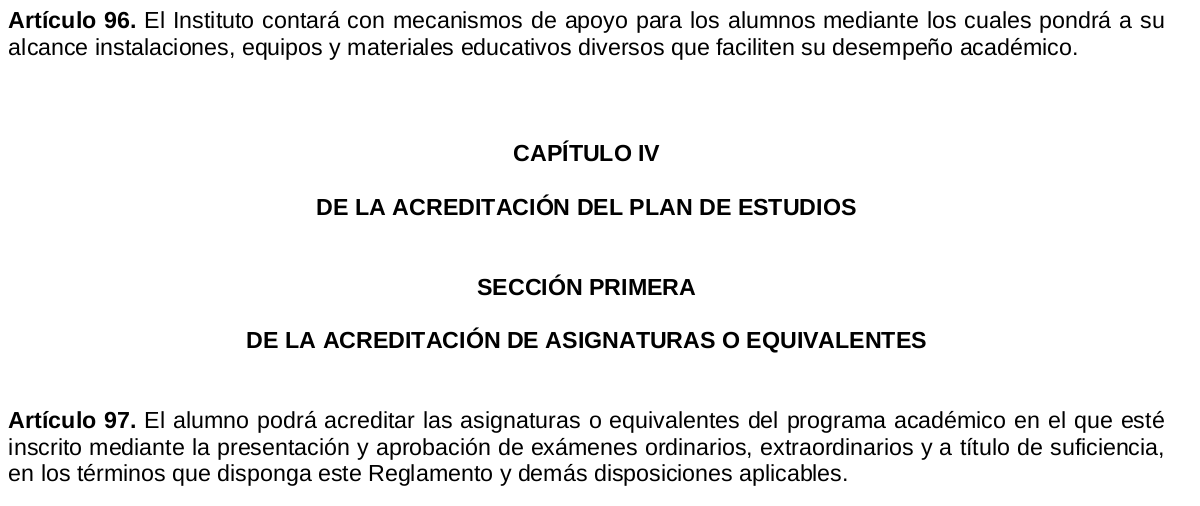
\includegraphics[scale=0.38]{6/ejemplo_reglamento_1}}
    \caption{Segmento del Reglamento Interno del Instituto Politécnico Nacional}
    \label{fig:ejemplo_1_reglamento_interno}
\end{figure}

\begin{figure}[ht]
    \centering
    \fbox{
\includegraphics[scale=0.39]{6/ejemplo_reglamento_2}}
    \caption{Segmento del Reglamento Orgánico del Instituto Politécnico Nacional}
    \label{fig:ejemplo_2_reglamento_organico}
\end{figure}

\begin{figure}[ht]
    \centering
    \fbox{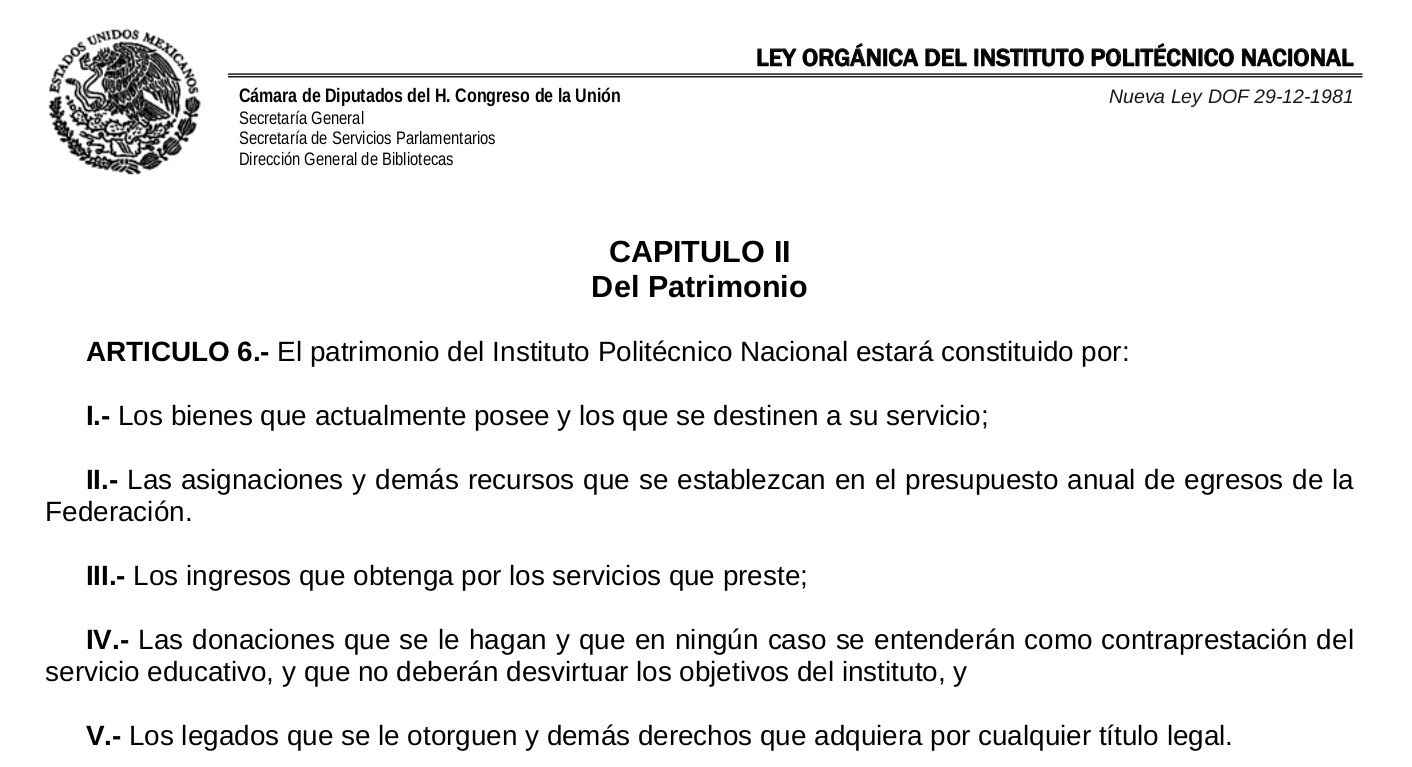
\includegraphics[scale=0.32]{6/ejemplo_reglamento_3}}
    \caption{Segmento de la Ley Orgánica del Instituto Politécnico Nacional}
    \label{fig:ejemplo_3_ley_organica}
\end{figure}

El problema general es este: la figura \ref{fig:ejemplo_1_reglamento_interno} muestra una manera muy sencilla de organización textual de la información, pero difiere mucho en cuanto a la organización de contenido de la figura \ref{fig:ejemplo_2_reglamento_organico}. Mas aún, la figura \ref{fig:ejemplo_3_ley_organica} añade a la estructura de la página una cabecera con nombres de una institución y sus direcciones internas, las cuáles son irrelevantes en cuanto al contenido normativo de nuestro interés.
 
Por lo tanto, podemos concluir que un estándar de división estructural normativa no es suficiente en sí, sino también \textbf{se debe estandarizar la forma en cómo se representan esos datos cuando se almacenan}. Esto es un problema de \textbf{serialización} de datos en la que no existe un formato unificado semántico. Se debe extraer esta información para posteriormente unificar su formato. Esto es el siguiente paso de la preparación del texto.

A pesar de que son relativamente pocos documentos, la cantidad de texto contenido dentro de ellos es grande como para extraer de manera manual. Sin embargo, para este trabajo terminal se ha decidido \textbf{extraer el texto a mano}. Este método es muy inconveniente por diversas razones. La principal razón que se considera en el desarrollo de este trabajo terminal es por el esfuerzo manual requerido, el cuál hace que el proceso sea propenso a errores. Como consecuencia esto también la cantidad de tiempo invertida en desarrollar este trabajo terminal.

Sin embargo, si se depende de una herramienta que extraiga texto automática mente, resulta en incongruencias como el siguiente segmento de texto extraído de la figura \ref{fig:ejemplo_2_reglamento_organico}:

\begin{quote}
    \textbf{Artículo 10.} En caso de que algún miembro del person-gación, al desarrollo y fomento tecnoloógico y empre-nal del Instituto reciba el nombramiento de directivo en sarial, o unidad educativa vinculada a ciencia, tecnología...
\end{quote}

Esto es debido a que la organización de texto no es la misma que la organización visual de un documento PDF. En este caso, la herramienta de extracción de PDF lo hizo por cada renglón de la página, sin importar que el documento estuviera dividido en dos columnas.

\newpage
\subsubsection{Formato de Documento Normativo de Entrada}

Entonces necesitamos que el documento venga en formato TXT, y que cada \textbf{título}, \textbf{sección}, \textbf{capítulo} y \textbf{artículo} venga separado por dos saltos de línea (\textbackslash n\textbackslash n). Tambien el texto y el nivel estructural debe ser separado con un guin (-) o un punto (.).

\begin{quote}
    \textbf{Capítulo Primero} - Disposiciones Generales
    
    \textbf{Artículo 1}. Las disposiciones del presente Reglamento son de observancia general y obligatoria en el Instituto Politécnico Nacional.
    
    \textbf{Artículo 2}. Este ordenamiento tiene por objeto establecer las condiciones que regulan el ingreso, la trayectoria escolar, la permanencia y el egreso de alumnos que cursen algún programa académico de los niveles medio superior, superior y posgrado, así como de los usuarios de todos aquellos programas que se ofrezcan para complementar su formación y con fines de capacitación, actualización técnica y profesional, formación empresarial, educación continua, y enseñanza de lenguas extranjeras en las unidades académicas, unidades de apoyo a la innovación educativa, unidades de apoyo a la investigación y al fomento y desarrollo empresarial y demás áreas referidas en el artículo 2 del Reglamento Orgánico, en las modalidades educativas que ofrece el Instituto Politécnico Nacional.
    
    \textbf{Artículo 3}. Para efectos del presente Reglamento se entenderá por:
    Academia: Al órgano constituido por profesores que tiene la finalidad de proponer, analizar, opinar, estructurar y evaluar el proceso educativo.
    ...
\end{quote}

Por ejemplo:

\begin{itemize}
    \item El primer elemento sería el capítulo primero, se separa el texto de su nivel mediante el guión. Posteriormente se introducen dos saltos de línea para separarlo del artículo 2. 
    \item El tercer elemento es el artículo 3. Este tiene mas de un párrafo, por lo que un solo salto de línea separa sus párrafos pero no lo separa del artículo siguiente hasta que encuentre los dos saltos de línea.
\end{itemize}

Los documentos normativos extraidos manualmente a un formato TXT se pueden encontrar en el siguiente repositorio: \url{https://github.com/AranGarcia/Shepard}.

\subsubsection{Estructura Propuesta}

Una vez obtenido el formato TXT de entrada, se utilizará como entrada al sistema para su almacenamiento en la base de conocimiento.

Para estructurar los reglamentos, se toma en cuenta la jerarquía de su división estructural mientras se mantenga el contenido textual así como la enumeeración. Es por eso que se propone la siguiente estructura:

\begin{itemize}
    \item \textbf{items}: arreglo de objetos con los siguientes atributos:
    
    \begin{itemize}
        \item \textbf{contenido}: objeto anidado recursivo
        
        \begin{itemize}
            \item \textbf{items}: ...
            \item \textbf{nivel}: ...
        \end{itemize}
        
        \item \textbf{enumeracion}: número de elemento de la división estructural
        \item \textbf{texto}: contenido textual del elemento
    \end{itemize}
    
    \item \textbf{nivel}: nombre del nivel de la división estructural
\end{itemize}

Este formato es para mantener una forma jerárquica inherente en los documentos normativos discutidos anteriormente y que se les denomina divisón estructural. Entonces se desarrollará un programa que dado un documento normativo TXT lo transforme a la estructura propuesta.

\begin{figure}
    \centering
    \lstinputlisting[language=yaml]{src/3/ejemplo-estructura.yaml}
    \caption{Estructura propuesta inicialmente para organizar texto mediante el lenguaje YAML.}
    \label{fig:estructura_propuesta}
\end{figure}

El programa que realiza esto se puede encontrar en el repositorio \url{https://github.com/AranGarcia/Cookie/tree/master/yamlizer}.